\documentclass[10pt]{beamer}
\usepackage[serbianc]{babel}
\usepackage[T2A]{fontenc}
\usepackage[utf8]{inputenc}
\usepackage{amssymb,amsmath,amsthm}
\usepackage{graphicx}
\usepackage{hyperref}
\graphicspath{ {./images/} }

\title{Algoritam sa fiksnim parametrom za nalaženje minimalne Menhetn mreže}
\author{Uroš Ševkušić}
\date{decembar 2022}
\institute{Univerzitet u Beogradu, Matematički fakultet}
\usetheme{Hannover}

\newtheorem{teo}{Teorema}

\begin{document}

\begin{frame}[plain]
\begin{center}
	\titlepage
\end{center}
\end{frame}

\begin{frame}{Uvod}
\begin{itemize}
    \item Autori rada:
    \begin{itemize}
        \item Kristijan Knauer (Christian Knauer) sa Instituta za informatiku pri Univerzitetu u Bajrojtu (Universität Bayreuth, Institut für Informatik)
        \item Adams Spilner (Adams Spillner) sa Instituta za matematiku i informatiku pri Univerzitetu u Grajfsvaldu (Universität Greifswald, Institut für Mathematik und Informatik)
    \end{itemize}
    \item Rad je objavljen 2011. godine u Journal of Computational Geometry
    \item Glavni rezultati rada su:
    \begin{itemize}
        \item konstrukcija algoritma za pronalaženje minimalne Menhetn mreže čija je vremenska složenost $O^*(2^{14h})$, gde je $h$ najmanji broj horizontalnih pravih koje pokrivaju skup $P$
        \item dokaz korektnosti algoritma
    \end{itemize}
\end{itemize}
\end{frame}

\begin{frame}{Osnovni pojmovi}
\begin{itemize}
        \item \textit{Menhetn mreža} za konačan skup tačaka $P$ u ravni je geometrijski graf $\mathcal{G} = (V, E)$ sa osobinama:
    \begin{itemize}
        \item $P \subseteq V$
        \item grane grafa su vertikalne ili horizontalne duži
        \item postoji put od bilo koje dve tačke $p$ i $q$ iz $P$ koji je jednak njihovom L1 rastojanju
        \item za svake dve grane $e_1 = \{p_1, q_1\}$ i $e_2 = \{p_2, q_2\}$, ako se duži $\overline{p_1, q_1}$ i $\overline{p_2, q_2}$ seku, njihov presek je $e_1 \cap e_2$
    \end{itemize}
    \item \textit{Dužina grane} $L(e)$ definiše se kao L1 rastojanje njenih krajnjih tačaka
    \item \textit{Dužina puta} $p$ sačinjenog od tačaka $p_1, p_2, \dots p_k$ definiše se kao \[ L(p) = \sum_{i = 1}^{k-1} L(\{p_i, p_{i+1}\}) \]
    \item Put $p$ je \textit{monoton} ako važi $L(p) = L(\{p_1, p_k\})$
    \item \textit{Dužina mreže} $\lambda(\mathcal{G})$ je zbir dužina svih grana u mreži
    \item Mreža je \textit{minimalna} ako je njena dužina najmanja od svih Menhetn mreža sa skupom tačaka $P$
\end{itemize}
\end{frame}

\begin{frame}{Opis algoritma - uvodni pojmovi}
\begin{itemize}
    \item Za svaku tačku $q$ ravni, označićemo njene $x$- i $y$- koordinate sa $x(q)$ i $y(q)$ respektivno
    \item Za skup tačaka $P$, sortiramo rastuće njene $x$-koordinate u niz $x_1, x_2, \dots x_l$
    \item Definišemo skup $X = \{ x(p) \mid p \in P \}$ i skupove $P_i = \{ p \in P \mid x(p) \leq x_i \}$ za sve $1 \leq i \leq l$
    \item Sortiramo tačke iz $P$ po $y$-koordinati u niz $y_1, y_2 \dots y_h$
    \item Neka je $Y = \{ y(p) \mid p \in P \}$ i neka su $L_j = \{ q \in \mathbb{R}^2 \mid y(q) = y_j \}$ za sve $1 \leq j \leq h$
    \item Tačke $v_{i, j} = (x_i, y_j)$ i $V_i = \{ v_{i, j} \mid 1 \leq j \leq h \}$
\end{itemize}
\end{frame}

\begin{frame}{Opis algoritma - uvodni pojmovi}
    \begin{itemize}
    \item Skup $R_{i, j}$ je najdešnja tačka $r_{i, j}$, ako takva postoji, u $P_i$ koja leži na $L_j$
    \item Za tačku $r_{i, j}$ se kaže da \textit{predstavlja} tačke $q$ takve da je $x(q) \leq x_i$ i $y(q) = y(r_{i, j})$
    \item Ako u Menhetn mreži za $P_i$ postoji monoton put od tačke $q'$ desno od $r_{i, j}$, onda postoji u toj mreži i monoton put od $q'$ do bilo koje tačke koju $r_{i, j}$ predstavlja
    \item To znači da, za svaku tačku $v_{i, j}$, kada želimo da proverimo ima li monoton put od nje do neke tačke $q$, dovoljno je posmatrati tačke $q$ iz skupa $S = \cup_{k = 1}^{h} R_{i, k}$
    \item Za Menhetn mrežu sa tačkama $P_i$, definišemo skup $R_i = \{ j \in \{1, 2, \dots, h\} \mid R_{i, j} \neq \varnothing \}$
    \item Za skup tačaka $P_i$, par $\Pi = ((A_1, \dots, A_h), (B_1, \dots, B_h))$ je \textit{prihvatljiv} ako je $A_j$ podskup od $\{j, j+1, \dots, h\} \cap R_i$ i $B_j$ podskup od $\{1, 2, \dots, j-1\} \cap R_i$ za sve $1 \leq j \leq h$
    \item Osnovna ideja je da se mreža za $P_i$ može opisati prihvatljivim parom kod kojeg su $A_j$ i $B_j$ indeksi $k$ onih tačaka za koje postoji monoton put od $v_{i, j}$ do $r_{i, k}$. Par za koje važi ovo svojstvo se naziva \textit{kanonski} i označava se sa $\pi(\mathcal{G})$
    \end{itemize}
\end{frame}

\begin{frame}{Algoritam}
    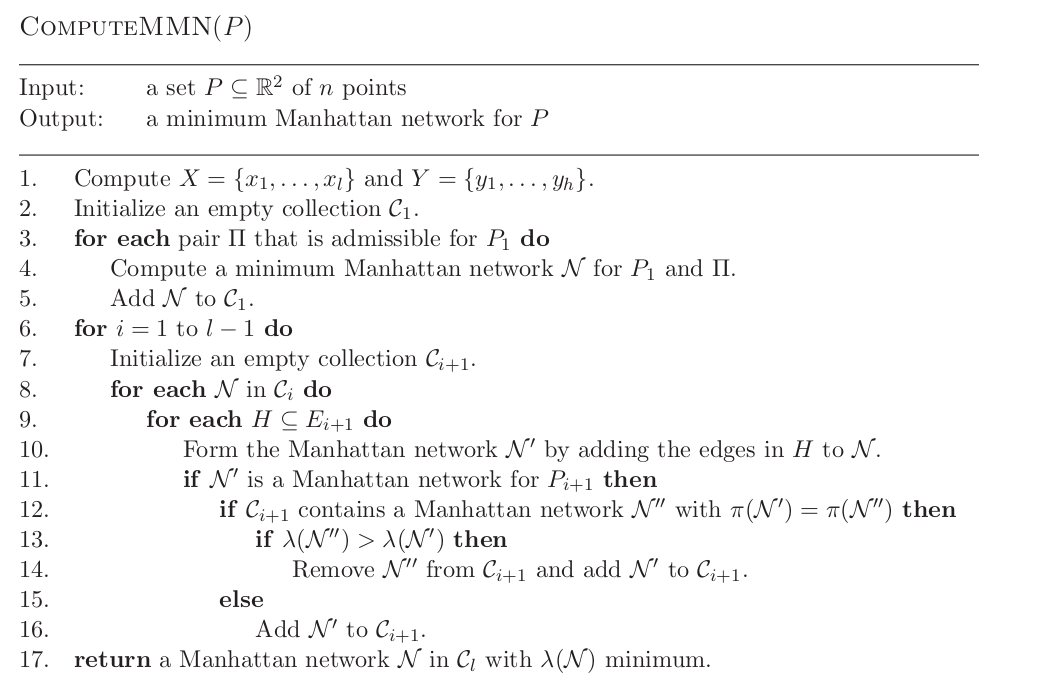
\includegraphics[scale=0.25]{images/MMN.png}
    \centering
\end{frame}

\begin{frame}{Algoritam}
    \begin{itemize}
        \item Algoritam radi iterativno - grade se kolekcije $\mathcal{C}_i$ Menhetn mreža za skupove $P_i$
        \item Algoritam će na kraju iz kolekcije $C_l$ izdvojiti najjeftiniju mrežu i vratiti je kao rezultat
        \item Ispostaviće se da je algoritam korektan, tj. da je rezultat algoritma zaista minimalna Menhetn mreža za $P$
        \item Prvi korak algoritma izgleda ovako:
        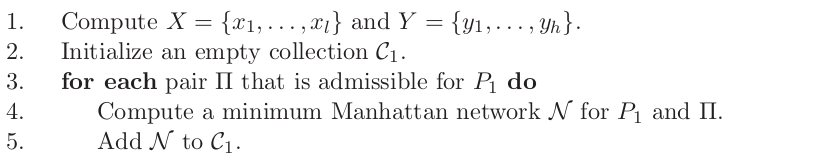
\includegraphics[scale=0.25]{images/korak1.png}
        \item Na samom početku algoritma, računamo skupove $X$ i $Y$
        \item Zatim se gradi kolekcija $C_1$
        \item Sve tačke iz $P_1$ su na istoj pravoj, pa je dovoljno samo povezati ih vertikalnim dužima da bi se napravila Menhetn mreža
        \item Tako izgrađenu Menhetn mrežu ubacujemo u kolekciju $C_1$
    \end{itemize}
\end{frame}

\begin{frame}{Algoritam}
    \begin{itemize}
        \item Sledeća faza je građenje kolekcija $C_i$ za $i \geq 2$:
        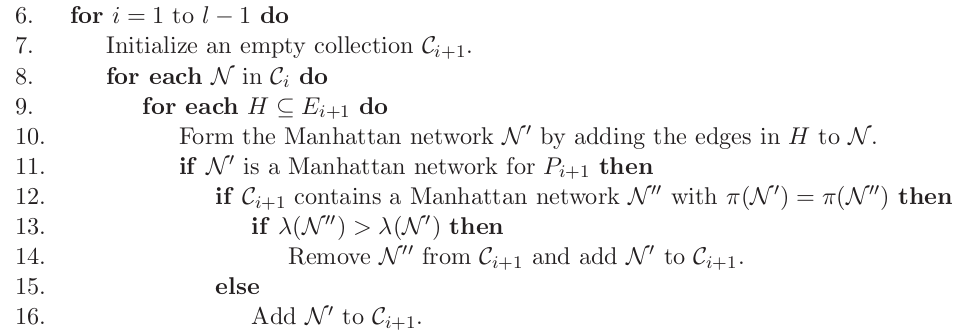
\includegraphics[scale = 0.25]{images/korak2.png}
        \item Za svaku mrežu iz prethodne kolekcije, pravimo nove mreže tako što dodajemo nove grane iz skupa grana $E_{i+1}$ u nju
        \item Skup grana $E_{i+1}$ čine grane $\{v_{i, j}, v_{i+1, j}\}$ i $\{v_{i+1, j}, v_{i+1, j+1}\}$
        \item Potrebno je proveriti da li mreža ispunjava uslove Menhetn mreža
        \item Ako je nova mreža jeftinija od neke iz kolekcije sa istim \textit{kanonskim prihvatljivim parom}, onda možemo da izbacimo staru mrežu
    \end{itemize}
\end{frame}

\begin{frame}{Algoritam - ilustracija}
    \centering
    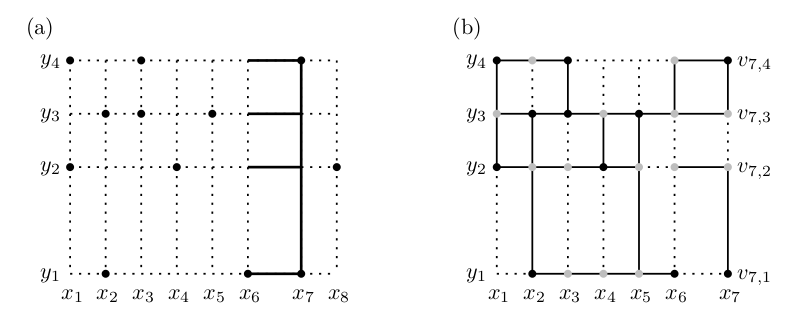
\includegraphics[scale = 0.3]{images/ilustracija.png}
    \begin{itemize}
        \item Podebljane linije na levoj slici prikazuju skup grana $E_7$
        \item Na desnoj slici smo neke od tih grana izabrali za novu mrežu
        \item Rezultujuća mreža u ovom koraku nije ispala Menhetn mreža
    \end{itemize}
\end{frame}

\begin{frame}{Redundantni parovi}
\begin{itemize}
\item Da bismo dokazali korektnost algoritma, potrebno je uvesti još dva pojma
\item Kažemo da prihvatljivi par $\Pi$ čini $\Pi'$ \textit{redundantnim} ako je:
\begin{itemize}
    \item $A_j' \subseteq A_j$
    \item $B_j' \subseteq B_j$
    \item svaka minimalna Menhetn mreža za $P_i$ i $\Pi'$ je minimalna Menhetn mreža za $P_i$ i $\Pi$
\end{itemize}
    \item Za skup $P_i$, \textit{pokrivač} je skup $\mathcal{A}$ prihvatljivih parova takvih da za sve prihvatljive parove $\Pi$ za $P_i$, postoji prihvatljiv par $\Pi' \in \mathcal{A}$ takav da $\Pi'$ čini $\Pi$ redundantnim
\end{itemize}
\end{frame}

\begin{frame}{Dokaz korektnosti}
\begin{itemize}
    \item Na osnovu sledeće tri teoreme, izvodi se dokaz korektnosti algoritma:
    \begin{teo}
            Neka je $i$ takvo da je $1 \leq i \leq l-1$. Pretpostavimo da je $\mathcal{A}_i = \{ \pi(\mathcal{G}) \mid \mathcal{G} \in C_i \}$ pokrivač i za svako $\Pi \in \mathcal{A}_i$ postoji minimalna Menhetn mreža za $P_i$ i $\Pi$ u $C_i$. Tada, za svaki prihvatljivi par $\Pi'$ za $P_{i+1}$, postoji Menhetn mreža $\mathcal{G} \in C_i$ i skup $H \subseteq E_{i+1}$ takva da je mreža $\mathcal{G'}$, koja je nastala dodavanjem grana iz $H$ u $\mathcal{G}$, minimalna Menhetn mreža za $P_{i+1}$ i $\Pi'$.
        \end{teo}
        \begin{teo}
            Neka je $i$ takvo da je $1 \leq i \leq l$. Neka je $\Pi$ prihvatljiv par za $P_i$ i $\mathcal{G}$ minimalna Menhetn mreža za $P_i$ i $\Pi$. Tada $\pi(\mathcal{G})$ čini $\Pi$ redundantnim.
        \end{teo}
            \begin{teo}
        Za svako $C_i$, $\mathcal{A}_i$ je pokrivač i $C_i$ sadrži minimalnu Menhetn mrežu za $P_i$ i svaki prihvatljivi par $\Pi$. Specijalno, $C_l$ sadži minimalnun Menhetn mrežu za $P$.
    \end{teo}
\end{itemize}
\end{frame}

\begin{frame}{Složenost}
\begin{itemize}
    \item Vremenska složenost ovog algoritma je $O^*(2^{14h})$, tj. $O(2^{14h} r(|P|))$, gde je $r$ neki polinom
    \item Prostorna složenost je $O^*(2^{12h})$
    \item Dokaz je sproveden u nekoliko faza:
    \begin{enumerate}
        \item Skupovi $A_j$ i $B_j$ mogu se predstaviti pravougaonicima
        \item Definiše se \textit{kompatibilna šestorka}, struktura koja se sastoji od četiri niza i dva skupa i koja će opisati te pravougaonike
        \item Ispostavlja se da, za svako $\mathcal{A}_i$, postoji injektivno preslikavanje $\varphi$ iz $\mathcal{A}_i$ u skup kompatibilnih šestorki
        \item Veličina skupa kompatibilnih šestorki je $O^*(2^{12h})$
        \item Primetimo da je $|C_i| = |A_i|$, iz čega sledi da je prostorna složenost $O^*(2^{12h})$
        \item Primetimo da imamo ne više od $2^{2h}$ podskupova $H$ od $E_{i+1}$
        \item Vremenska složenost je $O^*(2^{2h \cdot 12h}) = O^*(2^{14h})$
    \end{enumerate}
\end{itemize}
    
\end{frame}

\end{document}